\documentclass{jarticle}

%%%%%%%%%%%%%%%%%%%%%%%%%%%%%%%%%%%%%%%%%%%%%%%%%%%%%%%%%%%%%%%%%%%%%%%%%%%
% packages
%%%%%%%%%%%%%%%%%%%%%%%%%%%%%%%%%%%%%%%%%%%%%%%%%%%%%%%%%%%%%%%%%%%%%%%%%%%
\usepackage{amsmath}
\usepackage{amssymb}
\usepackage{amsfonts}
\usepackage[dvipdfmx]{graphicx}
\usepackage[dvipdfmx]{color}
\usepackage{graphicx}
\usepackage{bm}
\usepackage[section]{placeins}
%\usepackage[demo]{graphicx}
\usepackage{subfig}

%%%%%%%%%%%%%%%%%%%%%%%%%%%%%%%%%%%%%%%%%%%%%%%%%%%%%%%%%%%%%%%%%%%%%%%%%%%
% format stuffs
%%%%%%%%%%%%%%%%%%%%%%%%%%%%%%%%%%%%%%%%%%%%%%%%%%%%%%%%%%%%%%%%%%%%%%%%%%%
\setlength{\oddsidemargin}{0.455cm} 
\setlength{\evensidemargin}{0.455cm} 
\setlength{\textwidth}{15.5cm} 
\setlength{\textheight}{22.54cm}
\setlength{\headheight}{0mm}
\setlength{\headsep}{0mm}
\setlength{\topskip}{0mm}
\setcounter{topnumber}{100}
\setcounter{bottomnumber}{100}
\setcounter{totalnumber}{100}
\renewcommand{\topfraction}{1.0}
\renewcommand{\bottomfraction}{1.0}
\renewcommand{\textfraction}{0.0}
\renewcommand{\floatpagefraction}{0.0}
\renewcommand{\baselinestretch}{1.0}
\pagestyle{empty}

%%%%%%%%%%%%%%%%%%%%%%%%%%%%%%%%%%%%%%%%%%%%%%%%%%%%%%%%%%%%%%%%%%%%%%%%%%%
% math symbols and commands
%%%%%%%%%%%%%%%%%%%%%%%%%%%%%%%%%%%%%%%%%%%%%%%%%%%%%%%%%%%%%%%%%%%%%%%%%%%
\newcommand{\eq}[1]{(\ref{#1})}
\newcommand{\mtx}[2]{\left[\begin{array}{#1} #2 \end{array}\right]}
\newcommand{\mycase}[1]{\left\{\begin{array}{ll} #1 \end{array} \right.}
\newcommand{\mb}[1]{\mbox{\boldmath$#1$}}
\newcommand{\lw}[1]{\smash{\lower2.ex\hbox{#1}}}
\newcommand{\zero}{\mathbf{0}}
\newcommand{\one}{\mathbf{1}}
\newcommand{\eps}{\varepsilon}

%%%%%%%%%%%%%%%%%%%%%%%%%%%%%%%%%%%%%%%%%%%%%%%%%%%%%%%%%%%%%%%%%%%%%%%%%%%
% colors
%%%%%%%%%%%%%%%%%%%%%%%%%%%%%%%%%%%%%%%%%%%%%%%%%%%%%%%%%%%%%%%%%%%%%%%%%%%
\newcommand{\myred}[1]{\textcolor{red}{#1}}
\newcommand{\myredbf}[1]{\textcolor{red}{\bf #1}}
\newcommand{\myblue}[1]{\textcolor{blue}{#1}}
\newcommand{\mybluebf}[1]{\textcolor{blue}{\bf #1}}
\newcommand{\mydarkblue}[1]{\textcolor[rgb]{0.0,0.0,0.5}{#1}}
\newcommand{\mygreen}[1]{\textcolor[rgb]{0.0,0.5,0.0}{#1}}
\newcommand{\mygreenbf}[1]{\textcolor[rgb]{0.0,0.5,0.0}{\bf #1}}
\newcommand{\mypurple}[1]{\textcolor[rgb]{0.5,0.0,0.5}{#1}}
\newcommand{\mypurplebf}[1]{\textcolor[rgb]{0.5,0.0,0.5}{\bf #1}}
\begin{document}
%%%%%%%%%%%%%%%%%%%%%%%%%%%%%%%%%%%%%%%%%%%%%%%%%%%%%%%%%%%%%%%%%%%%%%%%%%%
% ここからがレポートの記述
%%%%%%%%%%%%%%%%%%%%%%%%%%%%%%%%%%%%%%%%%%%%%%%%%%%%%%%%%%%%%%%%%%%%%%%%%%%

\begin{center} 
{\large \bf 知能プログラミング演習I 第3レポート}
\end{center} %
\begin{flushright}
  \today
\end{flushright}
\begin{flushright}
\hskip 1mm
学籍番号 % 学籍番号
29114154 \\
\hskip 1mm
氏名 % 氏名
PHAM DUY
\end{flushright} % Name

%%%%%%%%%%%%%%%%%%%%%%%%%%%%%%%%%%%%%%%%%%%%%%%%%%%%%%%%%%%%%%%%%%%%%%%%%%%
\section{実験設定}
\begin{itemize}
  \item 分類クラス数:10(0から9までの手書きの数字)
  \item 中間層の数:8
  \item 中間層ごとのユニット数と各中間層で用いた活性化関数は以下になる。
  \begin{enumerate}
  \item Conv2D-1\\
  出力するフィルタ (チャネル) の枚数:64、活性化関数:ReLU、畳み込みのカーネルの大きさ:3、ストライド数:(1,1)(デフォルト)、パディング数:"same" 
\item Conv2D-2\\
出力するフィルタ (チャネル) の枚数:64、活性化関数:ReLU、畳み込みのカーネルの大きさ:3、ストライド数:(3,3)、パディング数:"same" 
\item MaxPooling2D-1\\
プーリングのフィルタサイズ:(2,2)
\item Conv2D-3\\
出力するフィルタ (チャネル) の枚数:64、活性化関数:ReLU、畳み込みのカーネルの大きさ:3、ストライド数:(1,1)(デフォルト)、パディング数:"same" 
\item Conv2D-4\\
出力するフィルタ (チャネル) の枚数:64、活性化関数:ReLU、畳み込みのカーネルの大きさ:3、ストライド数:(1,1)(デフォルト)、パディング数:"same" 
\item MaxPooling2D-2\\
プーリングのフィルタサイズ:(2,2)
\item Flatten
\item Dense:ユニット数:128、活性化関数:ReLU
\item 最後の中間層から出力層への活性化関数:ソフトマックス関数
\end{enumerate}
  \item 誤差関数:クロスエントロピー
  \item パラメータの更新方法:adam
 \item 評価関数:accuracy
  \item エポック数:10
  \item バッチサイズ:100\\
\end{itemize}
\begin{figure}[h]
\centering
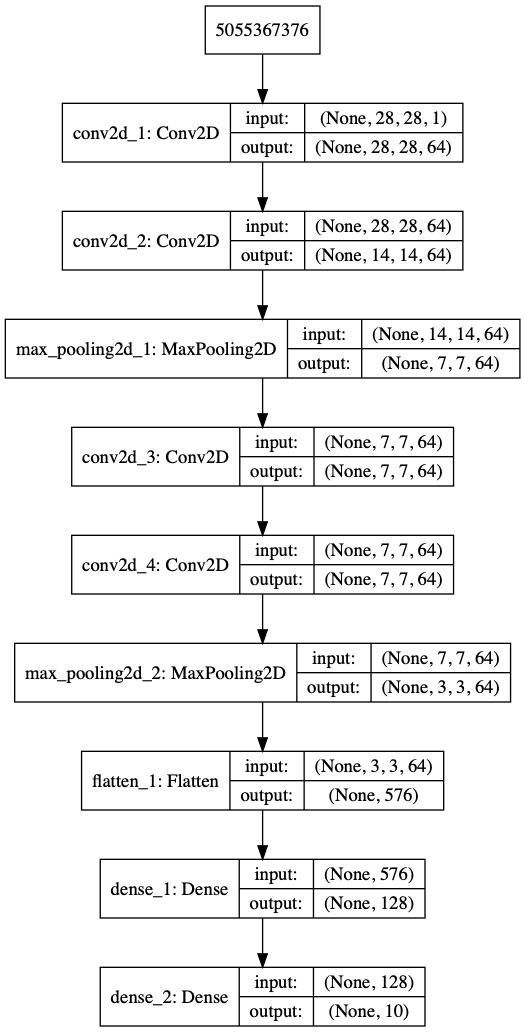
\includegraphics[height=20cm]{model.png}
\caption{設定したモデル}
\label{設定モデル}
\end{figure}
%%%%%%%%%%%%%%%%%%%%%%%%%%%%%%%%%%%%%%%%%%%%%%%%%%%%%%%%%%%%%%%%%%%%%%%%%%%


%%%%%%%%%%%%%%%%%%%%%%%%%%%%%%%%%%%%%%%%%%%%%%%%%%%%%%%%%%%%%%%%%%%%%%%%%%%
\clearpage
\section{結果}
解析結果は以下の図1、図2、図3で表す。
図1は訓練誤差とテスト誤差の推移を表す。図1の縦軸は誤差を表し、図1の横軸はデータのスキャン回数(epoch数)を表す。誤差が小さければ小さいほど良い。図2は訓練分類精度とテスト分類精度の推移を表す。図2の縦軸は分類精度を表し、横軸はデータのスキャン回数(epoch数)を表す。分類精度が高ければ高いほど良い。図3は分類結果の数を表す。図3の縦軸はデータの実際のラベルで、図3の横軸は予測結果である。
\begin{figure}[h]
\centering
\subfloat[誤差の推移]{{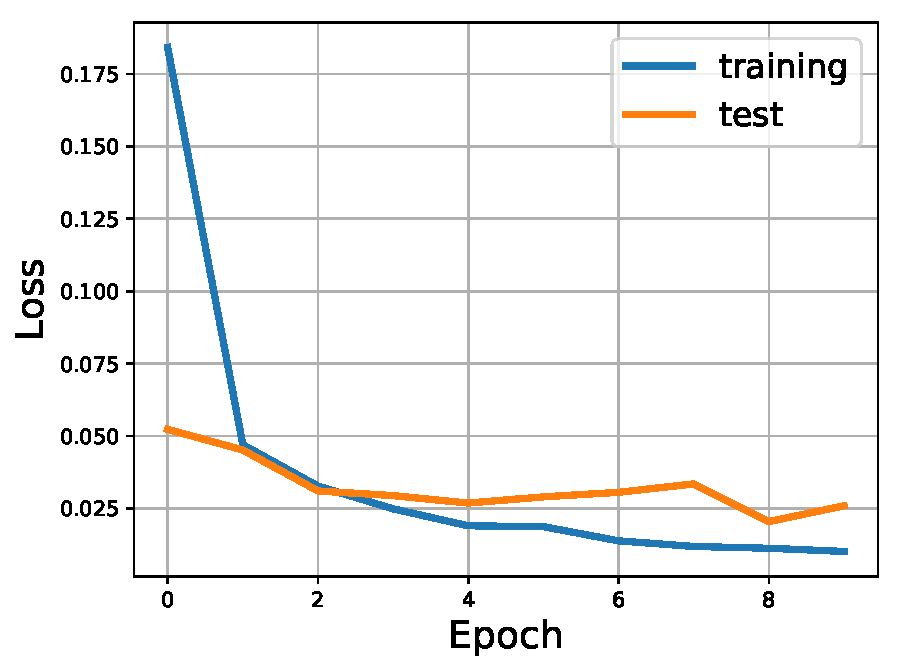
\includegraphics[width=7cm]{error.pdf} }}%
\qquad
\subfloat[精度の推移]{{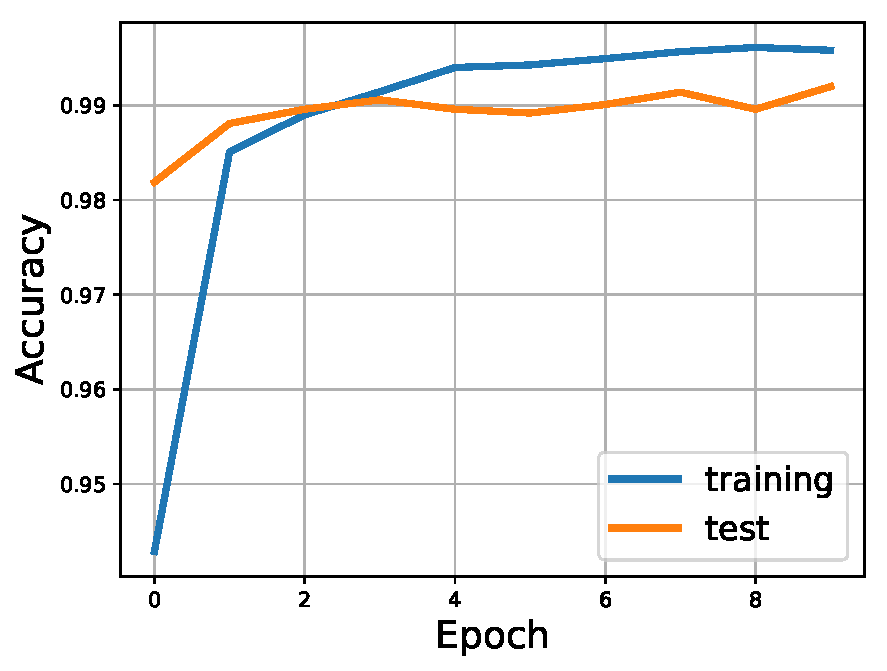
\includegraphics[width=7cm]{accuracy.pdf} }}%
\qquad
\subfloat[confusion martix]{{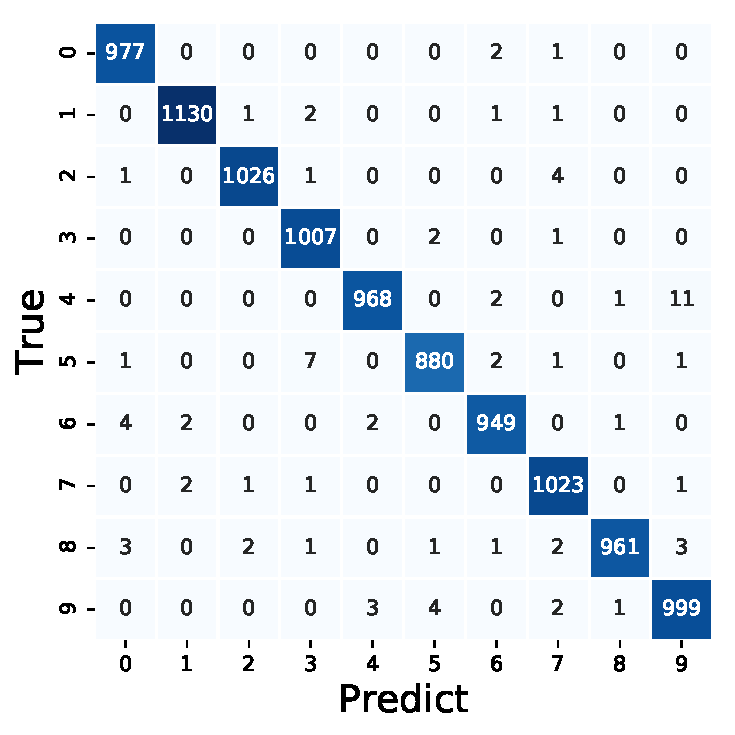
\includegraphics[width=8cm]{confusion.pdf} }}%
\caption{10エポックでの誤差関数の推移と分類精度の推移とconfusion matrix}%
\label{fig:example}%
\end{figure}

%%%%%%%%%%%%%%%%%%%%%%%%%%%%%%%%%%%%%%%%%%%%%%%%%%%%%%%%%%%%%%%%%%%%%%%%%%%
\clearpage
\section{考察}
以上の結果より、作成したモデルでデータのスキャン回数(epoch 数)をあげるに連れて訓練誤差と テスト誤差が減少している様子が確認できる。訓練誤差が急 激に減少している様子が見えるが、テスト誤差が徐々に減少してい る。このモデルの場合、未学習と過学習現象が見えていない。\\
confusion matrixの結果より、このモデルの分類精度は99.34\%に達していることがわかる。また、誤分類の例は以下の図3で表す。\\
今回に実装したCNNモデルによる分類精度は前回に実装したRNNモデルとDNNモデルによる分類精度より高いことがわかる。この点より、CNNモデルは手書きの数字の特徴をうまく抽出できると考えられる。
\begin{figure}[h]
\centering
\subfloat[7を2と誤って予測された例]{{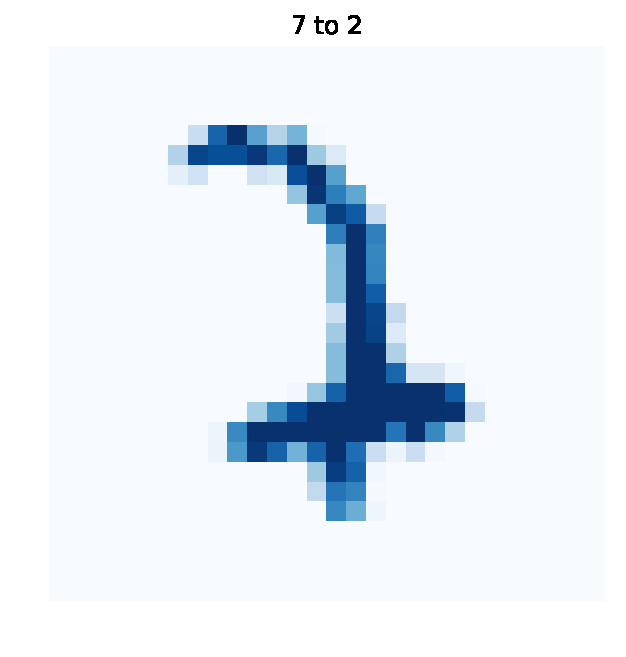
\includegraphics[width=7cm]{7to2.pdf} }}%
\qquad
\subfloat[9を4と誤って予測された例]{{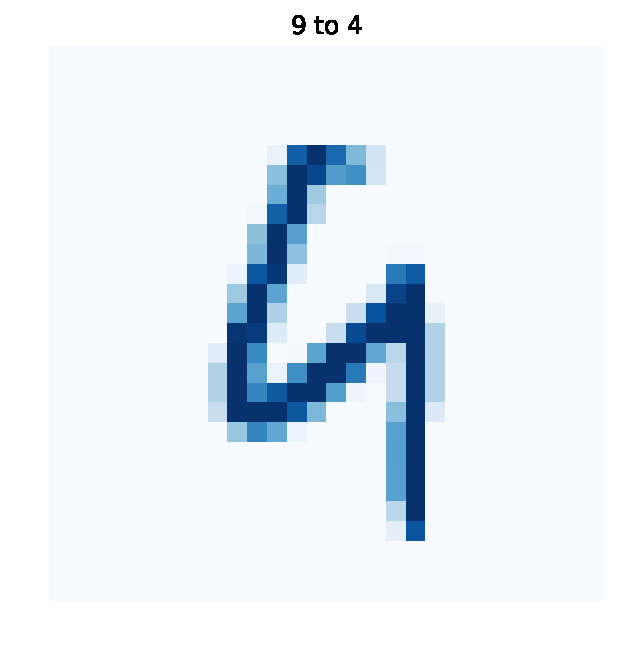
\includegraphics[width=7cm]{9to4.pdf} }}%
\caption{誤分類したデータの図示}%
\label{fig:example}%
\end{figure}


%%%%%%%%%%%%%%%%%%%%%%%%%%%%%%%%%%%%%%%%%%%%%%%%%%%%%%%%%%%%%%%%%%%%%%%%%%%
% ここまでがレポートの記述
%%%%%%%%%%%%%%%%%%%%%%%%%%%%%%%%%%%%%%%%%%%%%%%%%%%%%%%%%%%%%%%%%%%%%%%%%%%
\end{document}
